\begin{frame}[noframenumbering]
\frametitle{The Remy protocol synthesis procedure}
\begin{itemize}
\item<1-> Protocol: range-based rule table from \textit{state} to \textit{action}
\item<2-> State: Congestion signals tracked by the sender
\begin{itemize}
\item s\_ewma : EWMA over packet inter-transmit times
\item r\_ewma : EWMA over ACK inter-arrival times
\item rtt\_ratio: Ratio of RTT to minimum RTT
\item slow\_r\_ewma: Slower version of s\_ewma
\end{itemize}
\item<3-> Action: modify window, transmission rate
\begin{itemize}
\item Multiplier $m$ to current window
\item Increment $c$ to current window
\item Minimum inter-transmit time.
\end{itemize}
\end{itemize}
\end{frame}

\begin{frame}[noframenumbering]
\frametitle{The Remy protocol synthesis procedure}
\begin{enumerate}
\item Start with one rule: one action for all states
\item Optimize each action to maximize objective
\item Find most used rule
\item Median split that rule based on state usage
\item Repeat 2, 3, and 4 till you converge
\end{enumerate}
\end{frame}

\begin{frame}[noframenumbering]

\only<1>{\frametitle{One action for all states. Find the best value.}
\begin{centering}
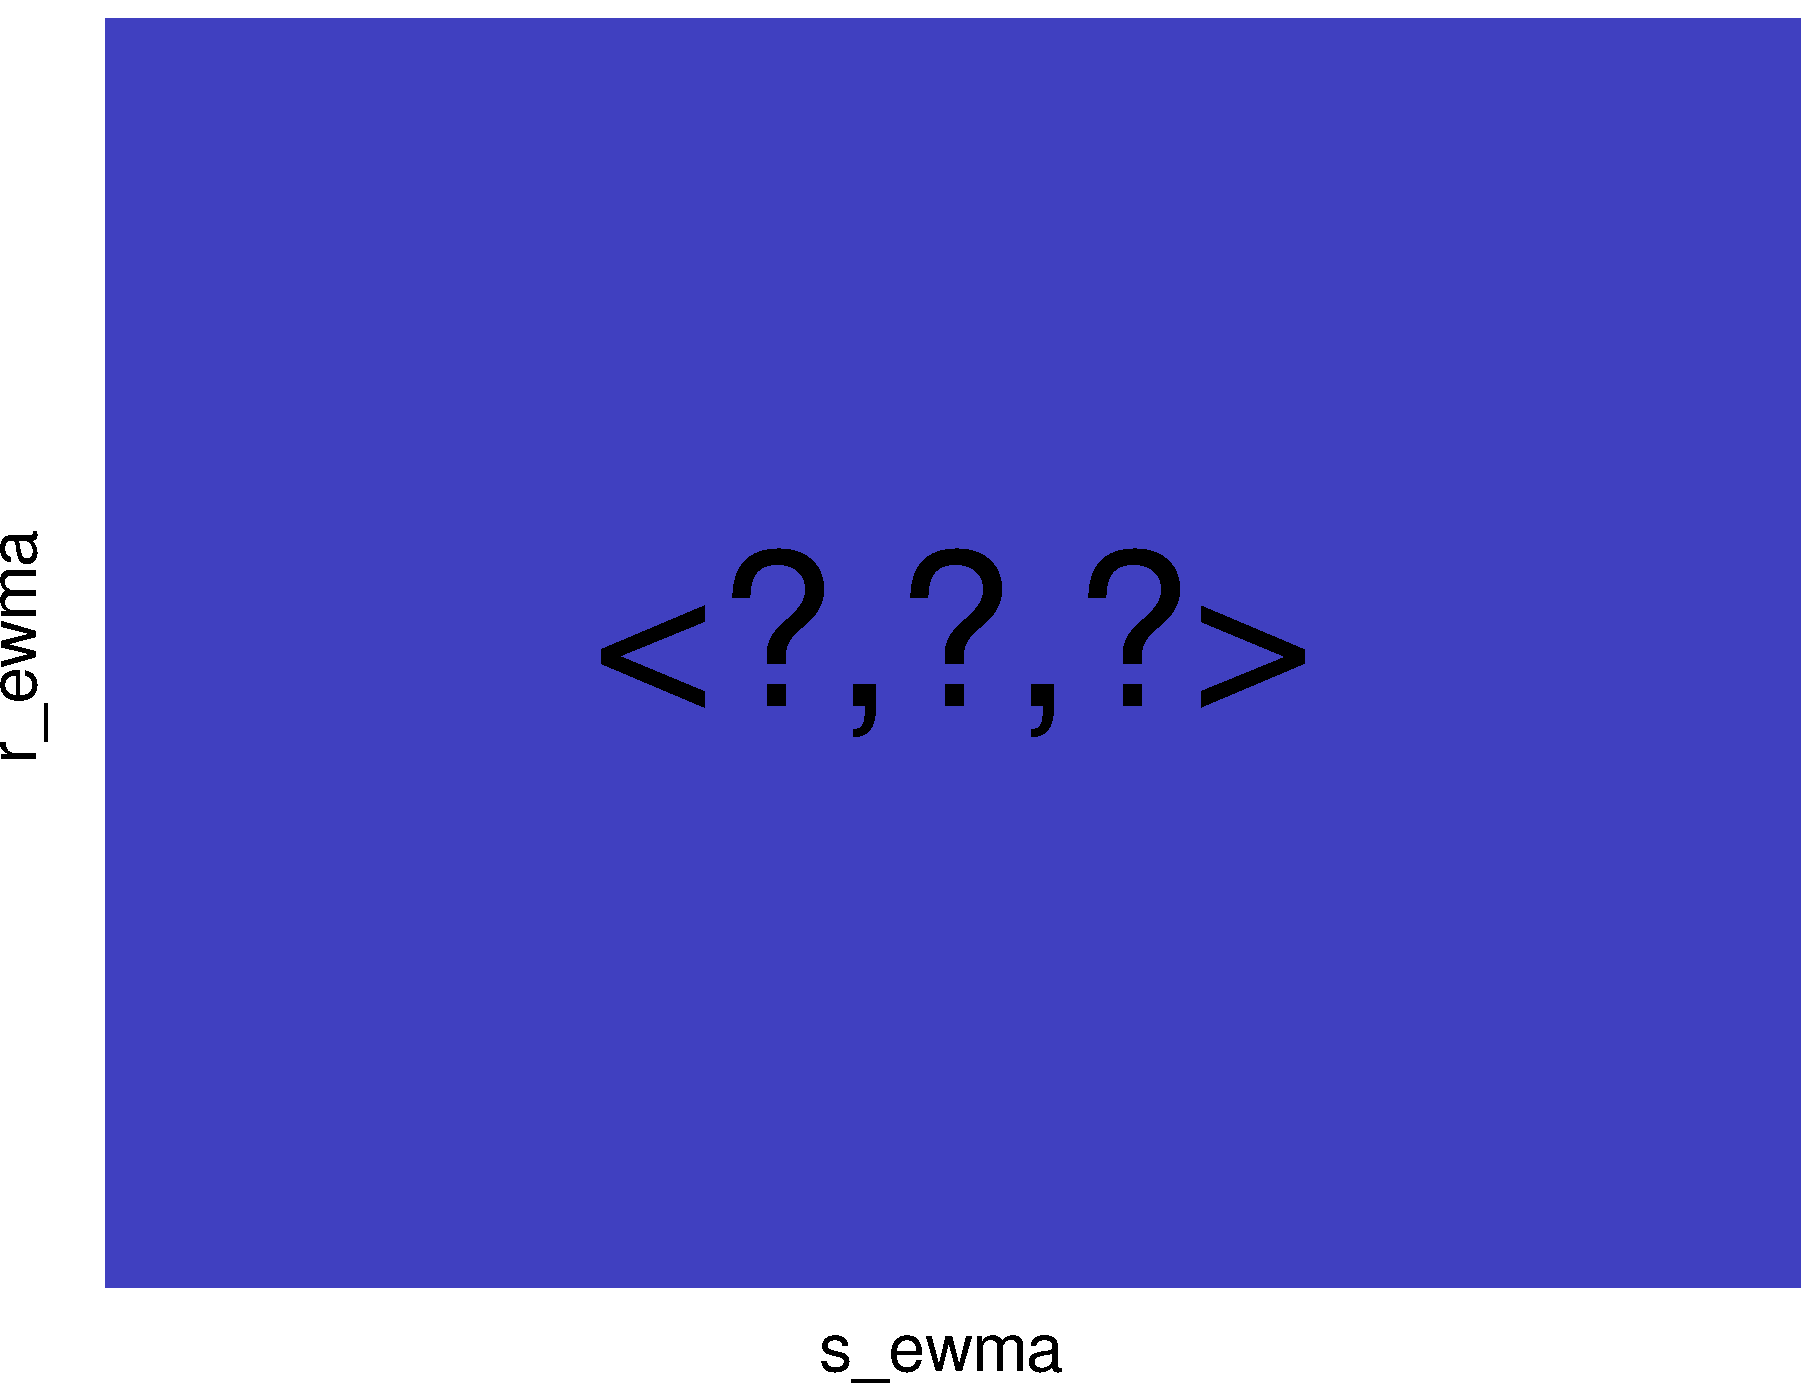
\includegraphics[width=9.25 cm]{remy-graph/graph/test0.pdf}

\end{centering}}
\only<2>{\frametitle{The best (single) action. Now split it on median.}
\begin{centering}
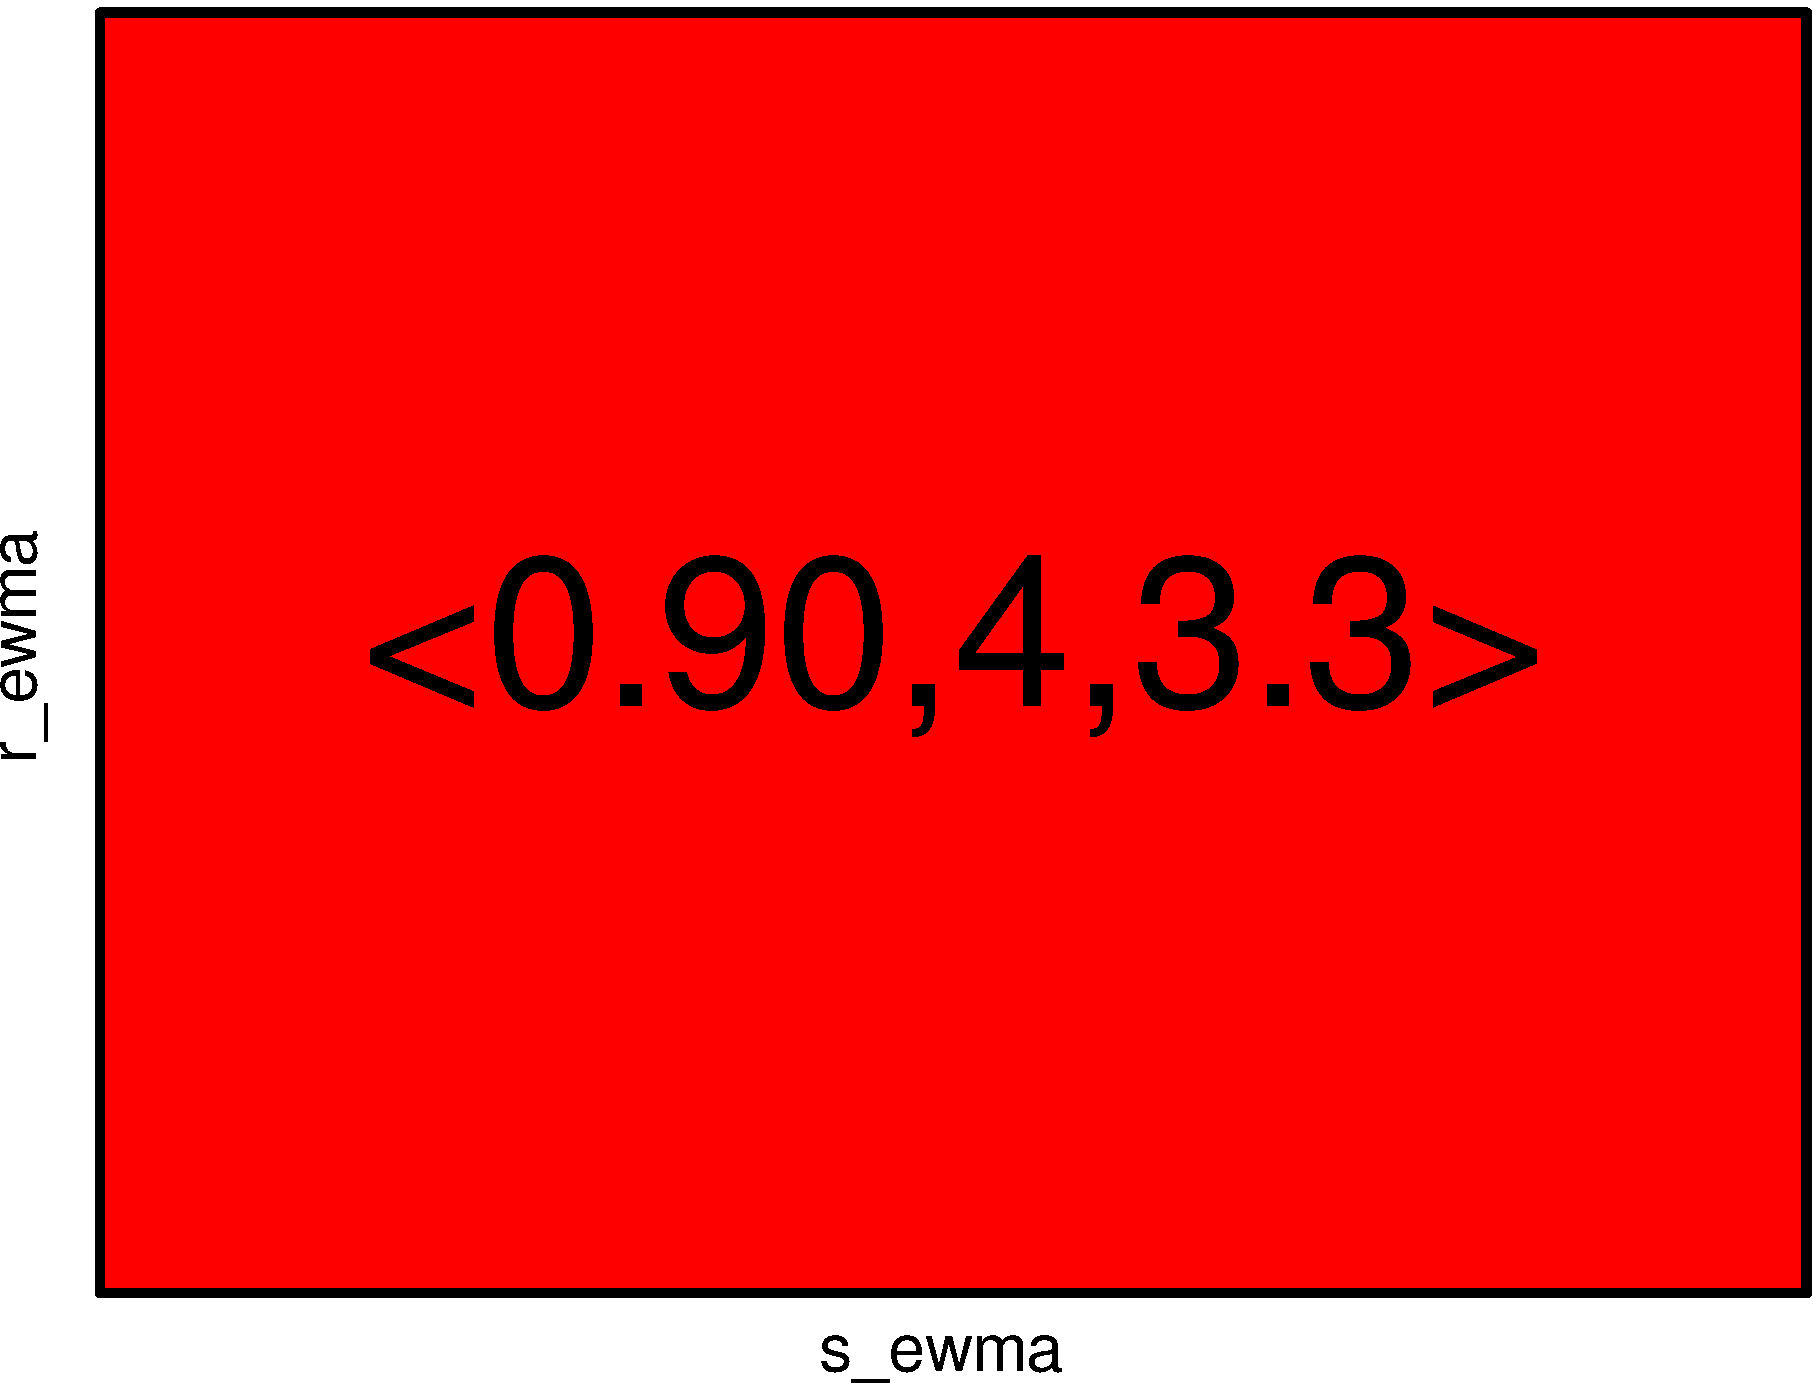
\includegraphics[width=9.25 cm]{remy-graph/graph/test1.pdf}

\end{centering}}

\only<3>{\frametitle{Simulate}
\begin{centering}
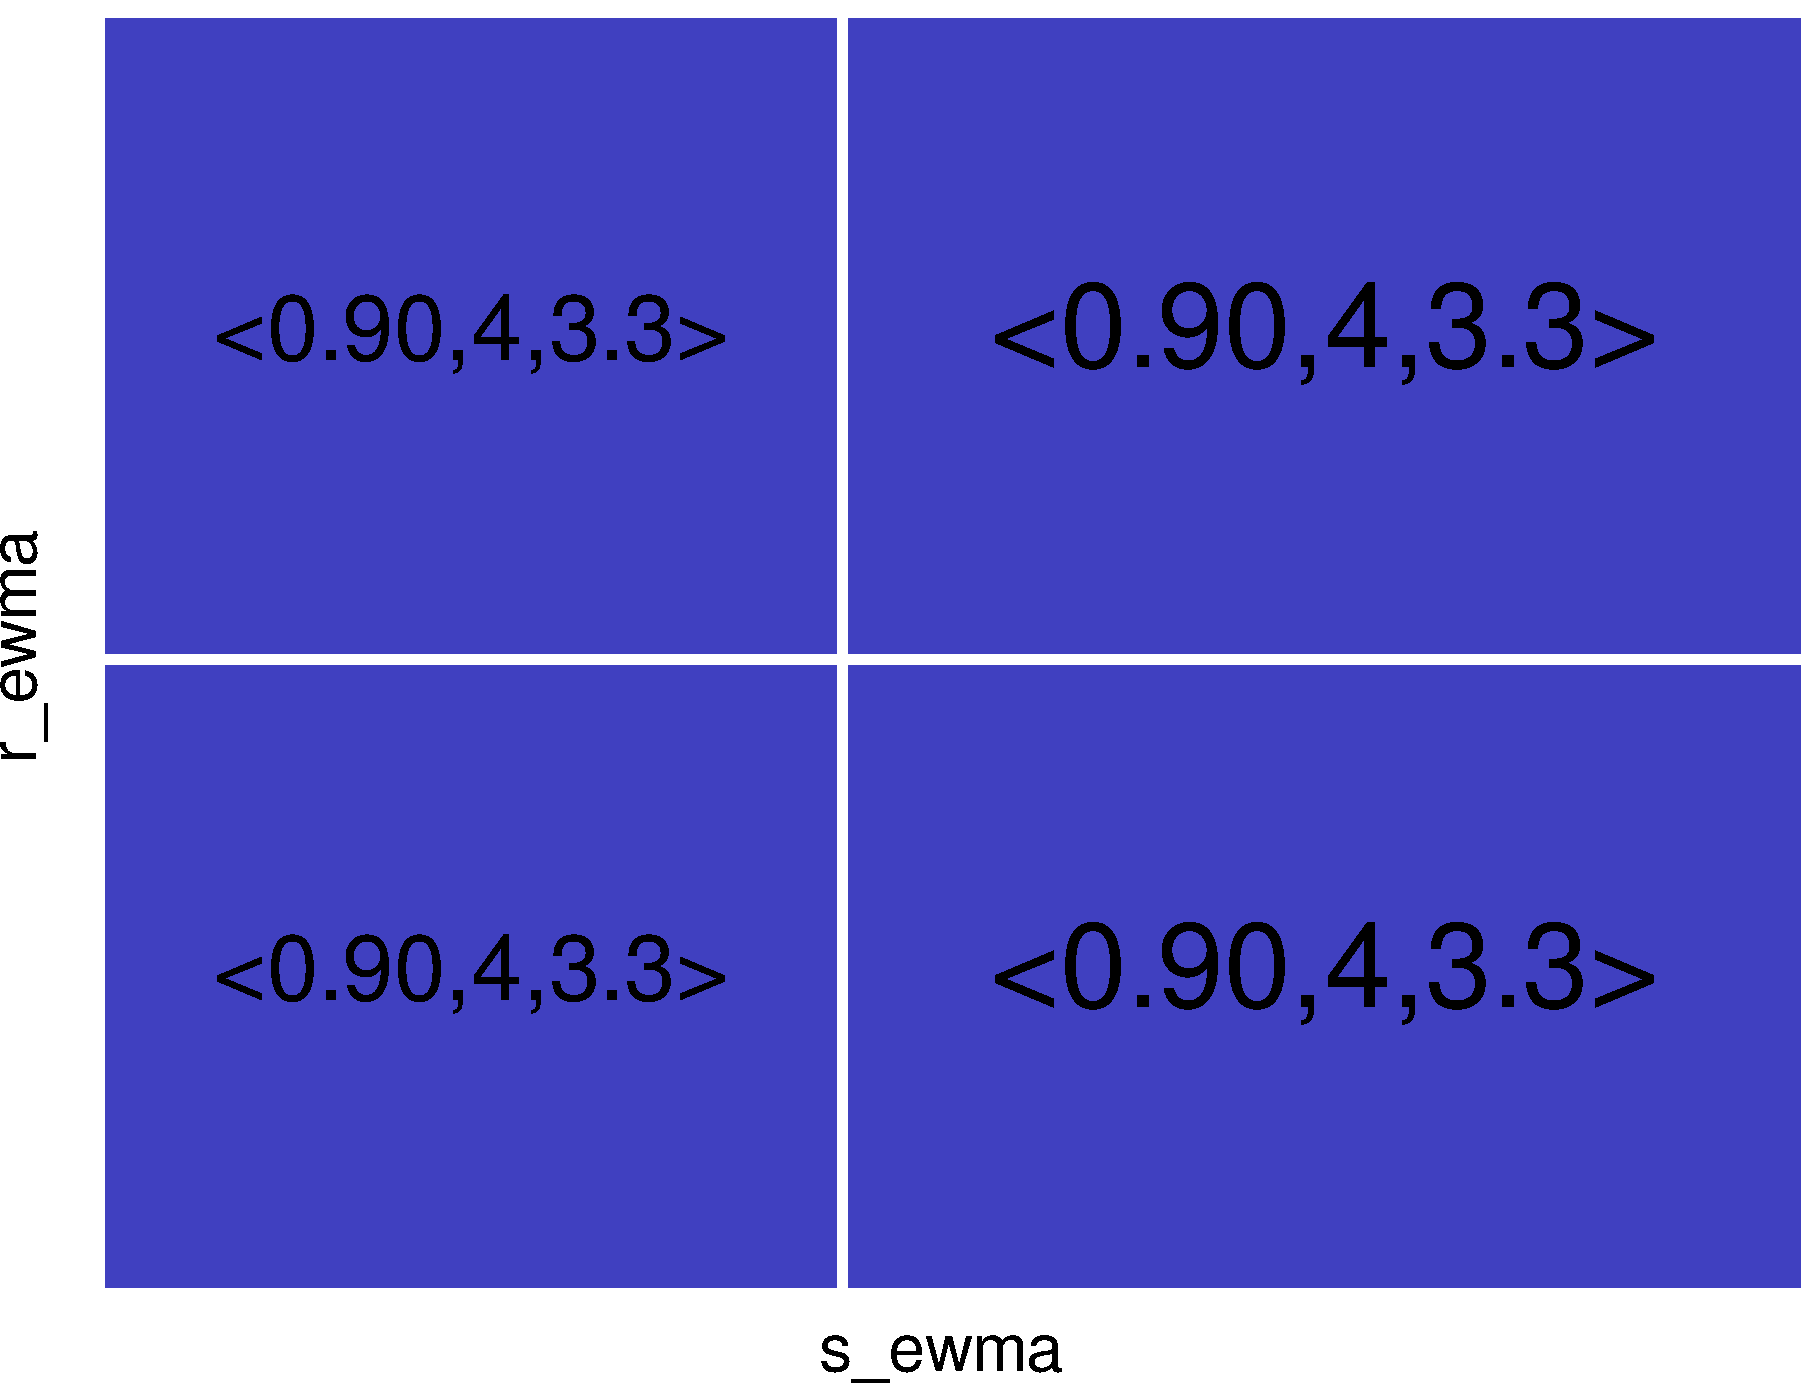
\includegraphics[width=9.25 cm]{remy-graph/graph/test2.pdf}

\end{centering}
}

\only<4>{\frametitle{Optimize each of the new actions}
\begin{centering}
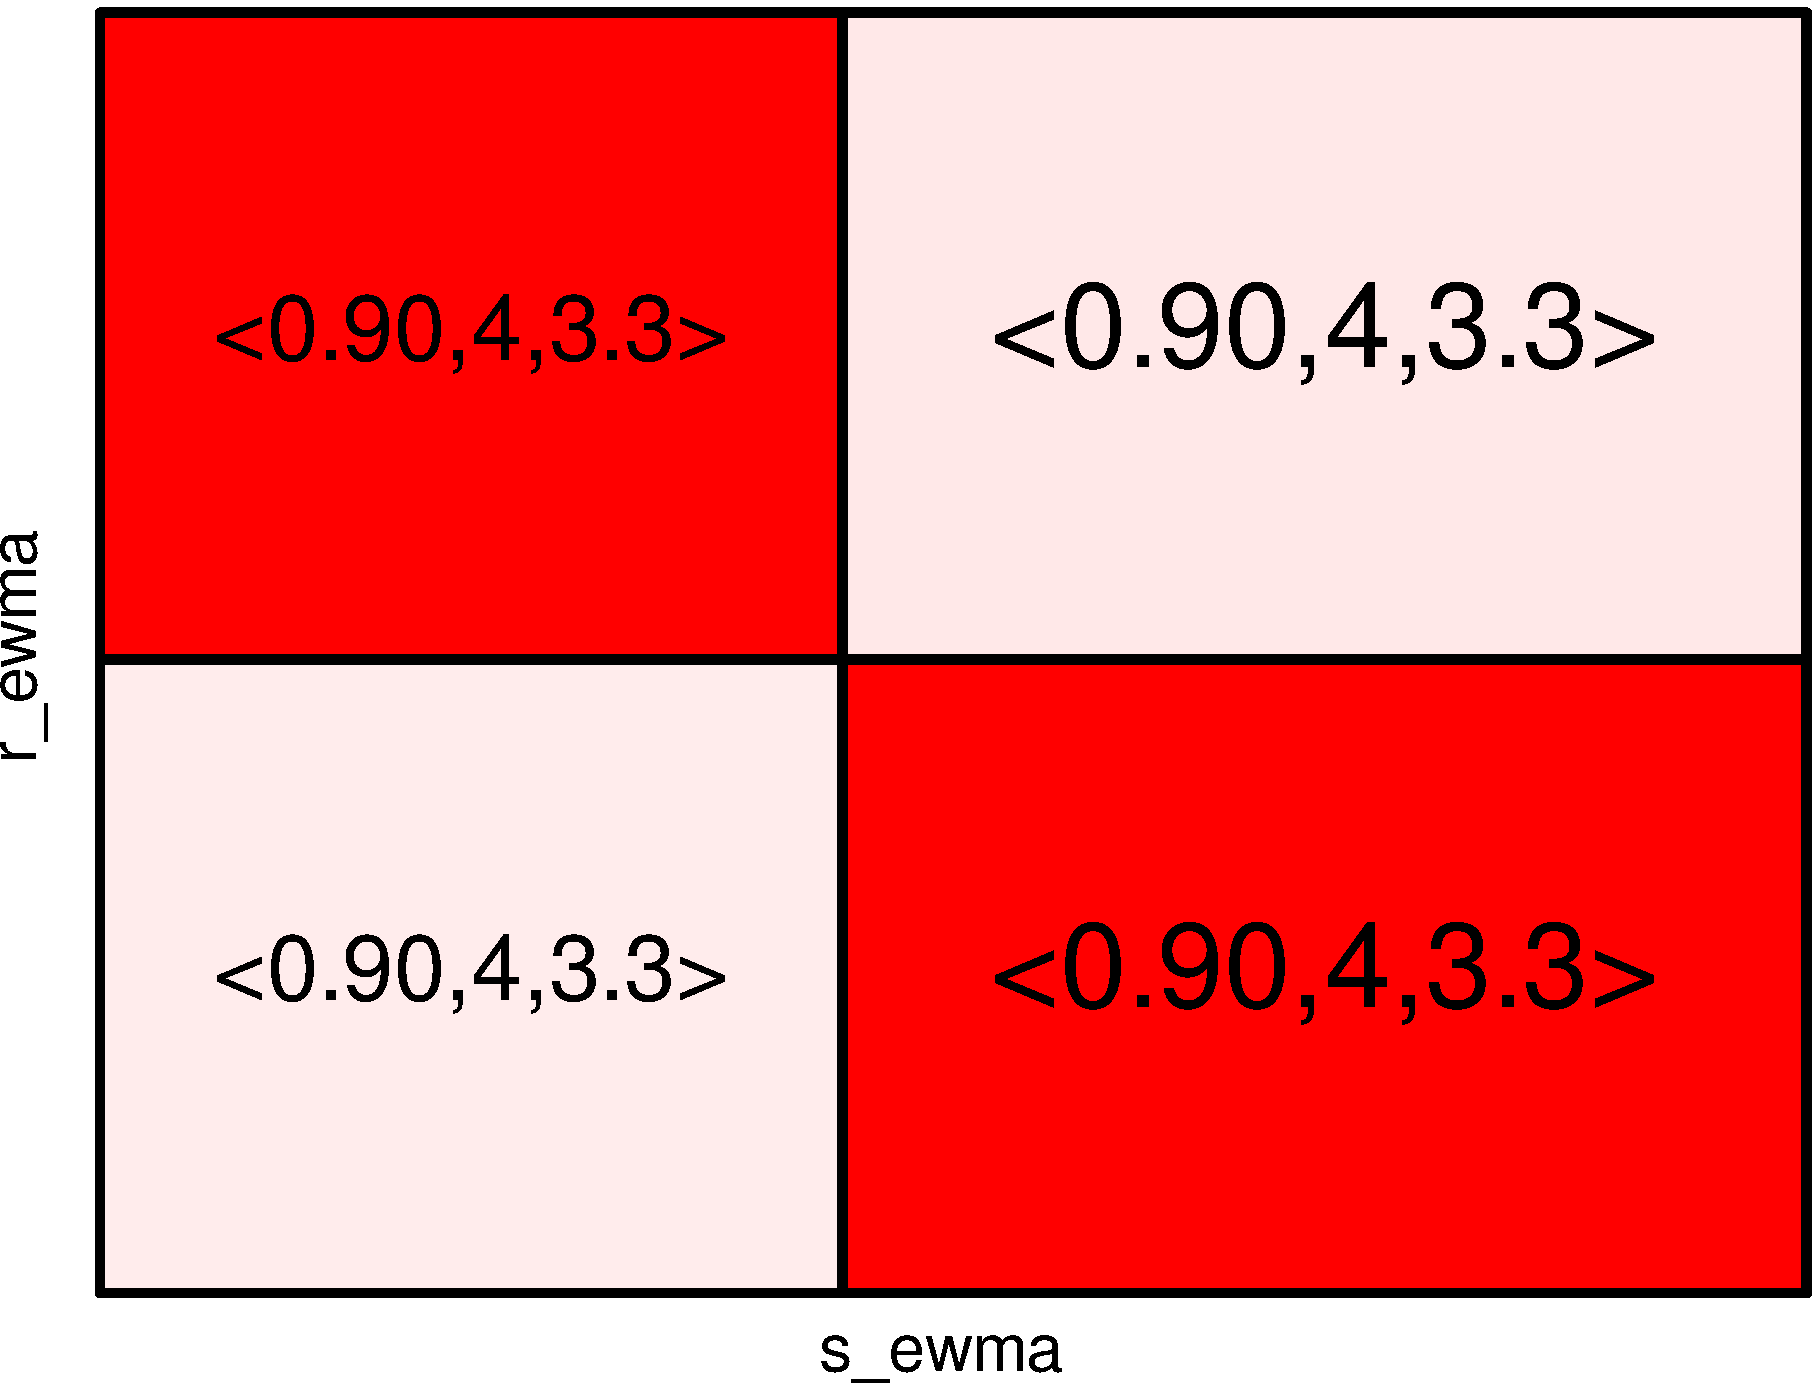
\includegraphics[width=9.25 cm]{remy-graph/graph/test3.pdf}

\end{centering}
}

\only<5>{\frametitle{Now split the most-used rule}
\begin{centering}
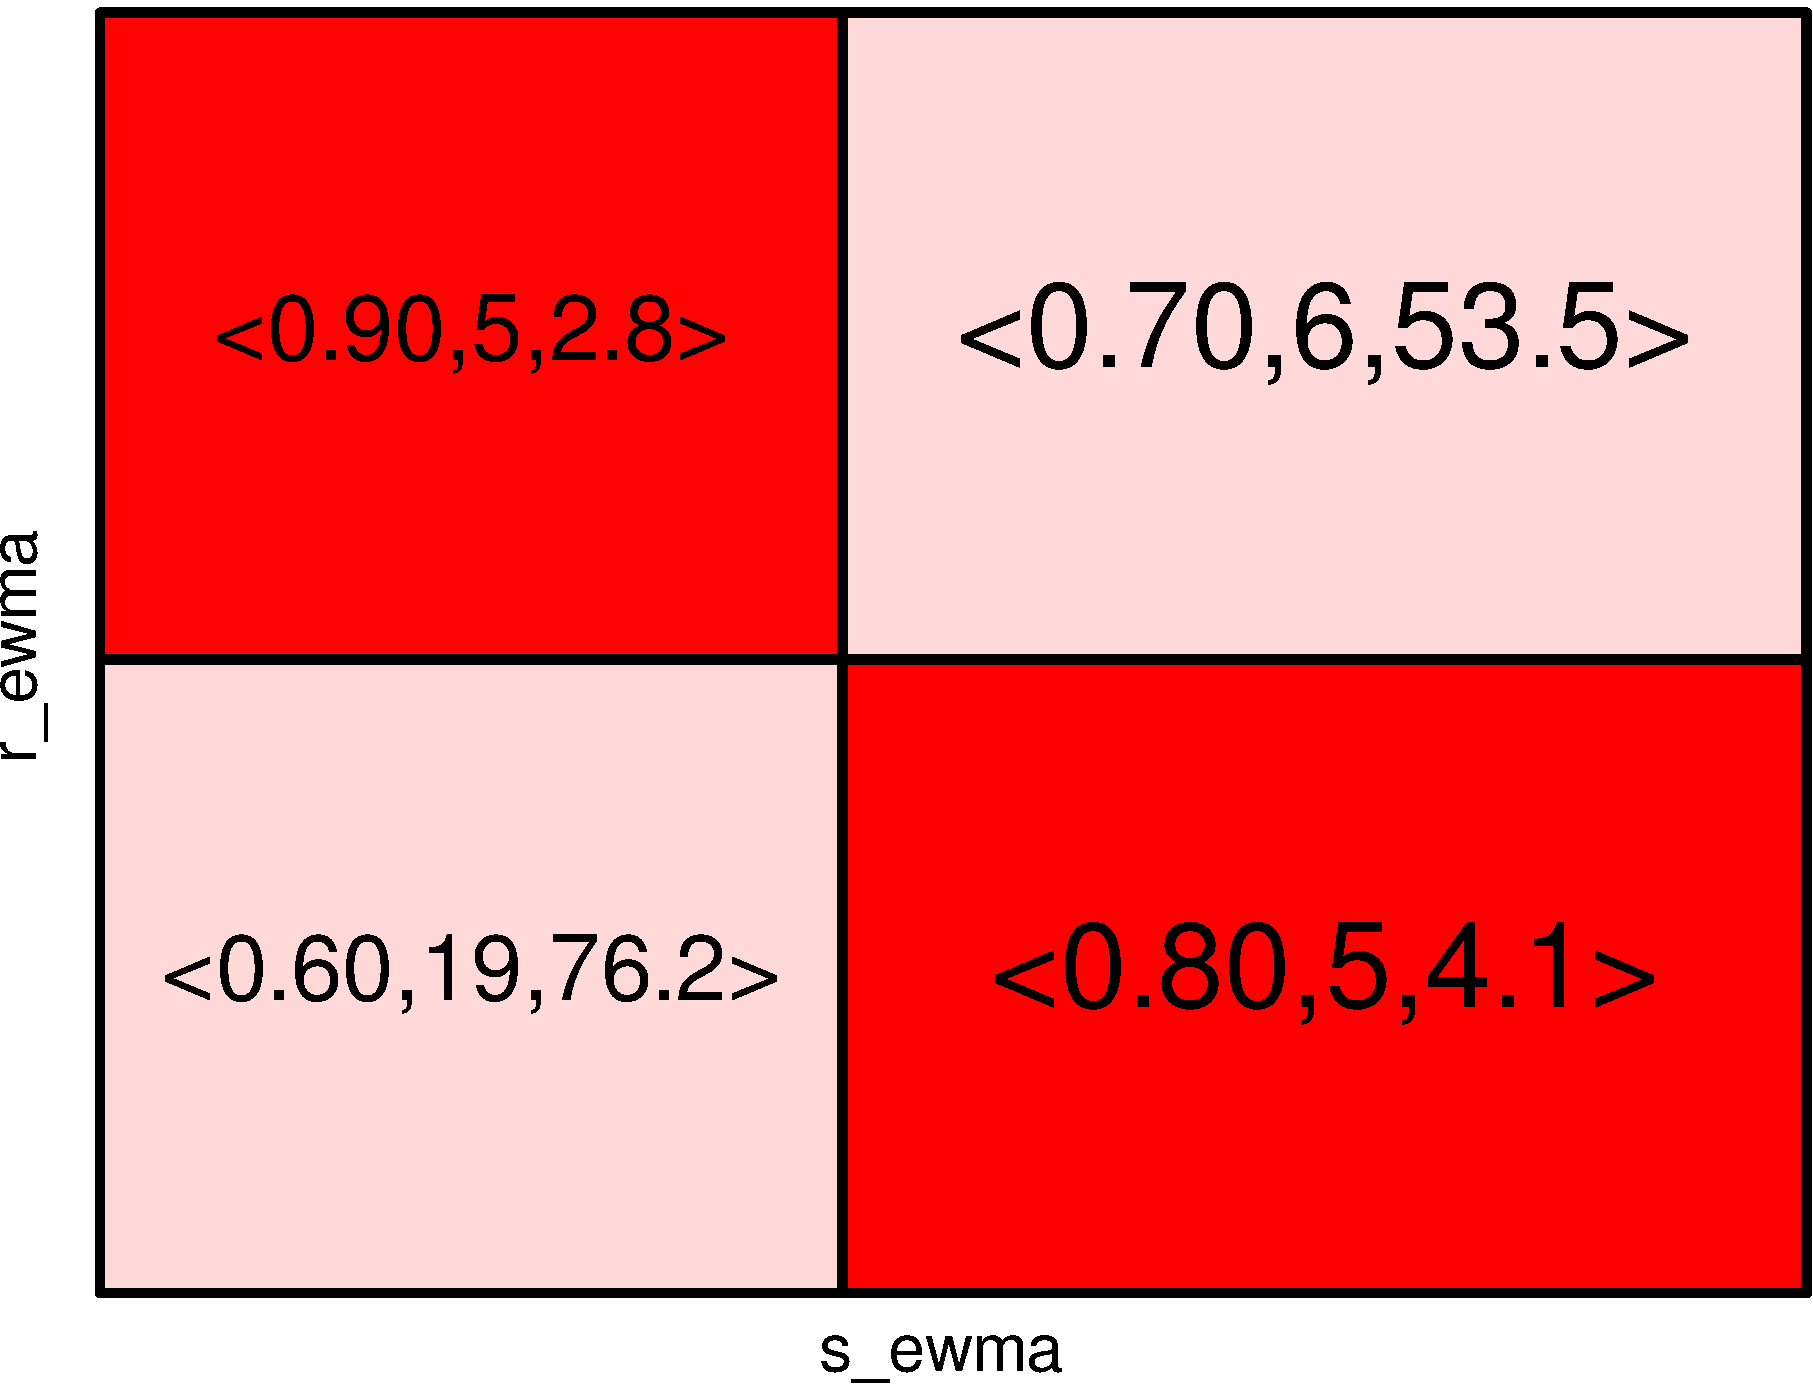
\includegraphics[width=9.25 cm]{remy-graph/graph/test4.pdf}

\end{centering}
}

\only<6>{\frametitle{Simulate}
\begin{centering}
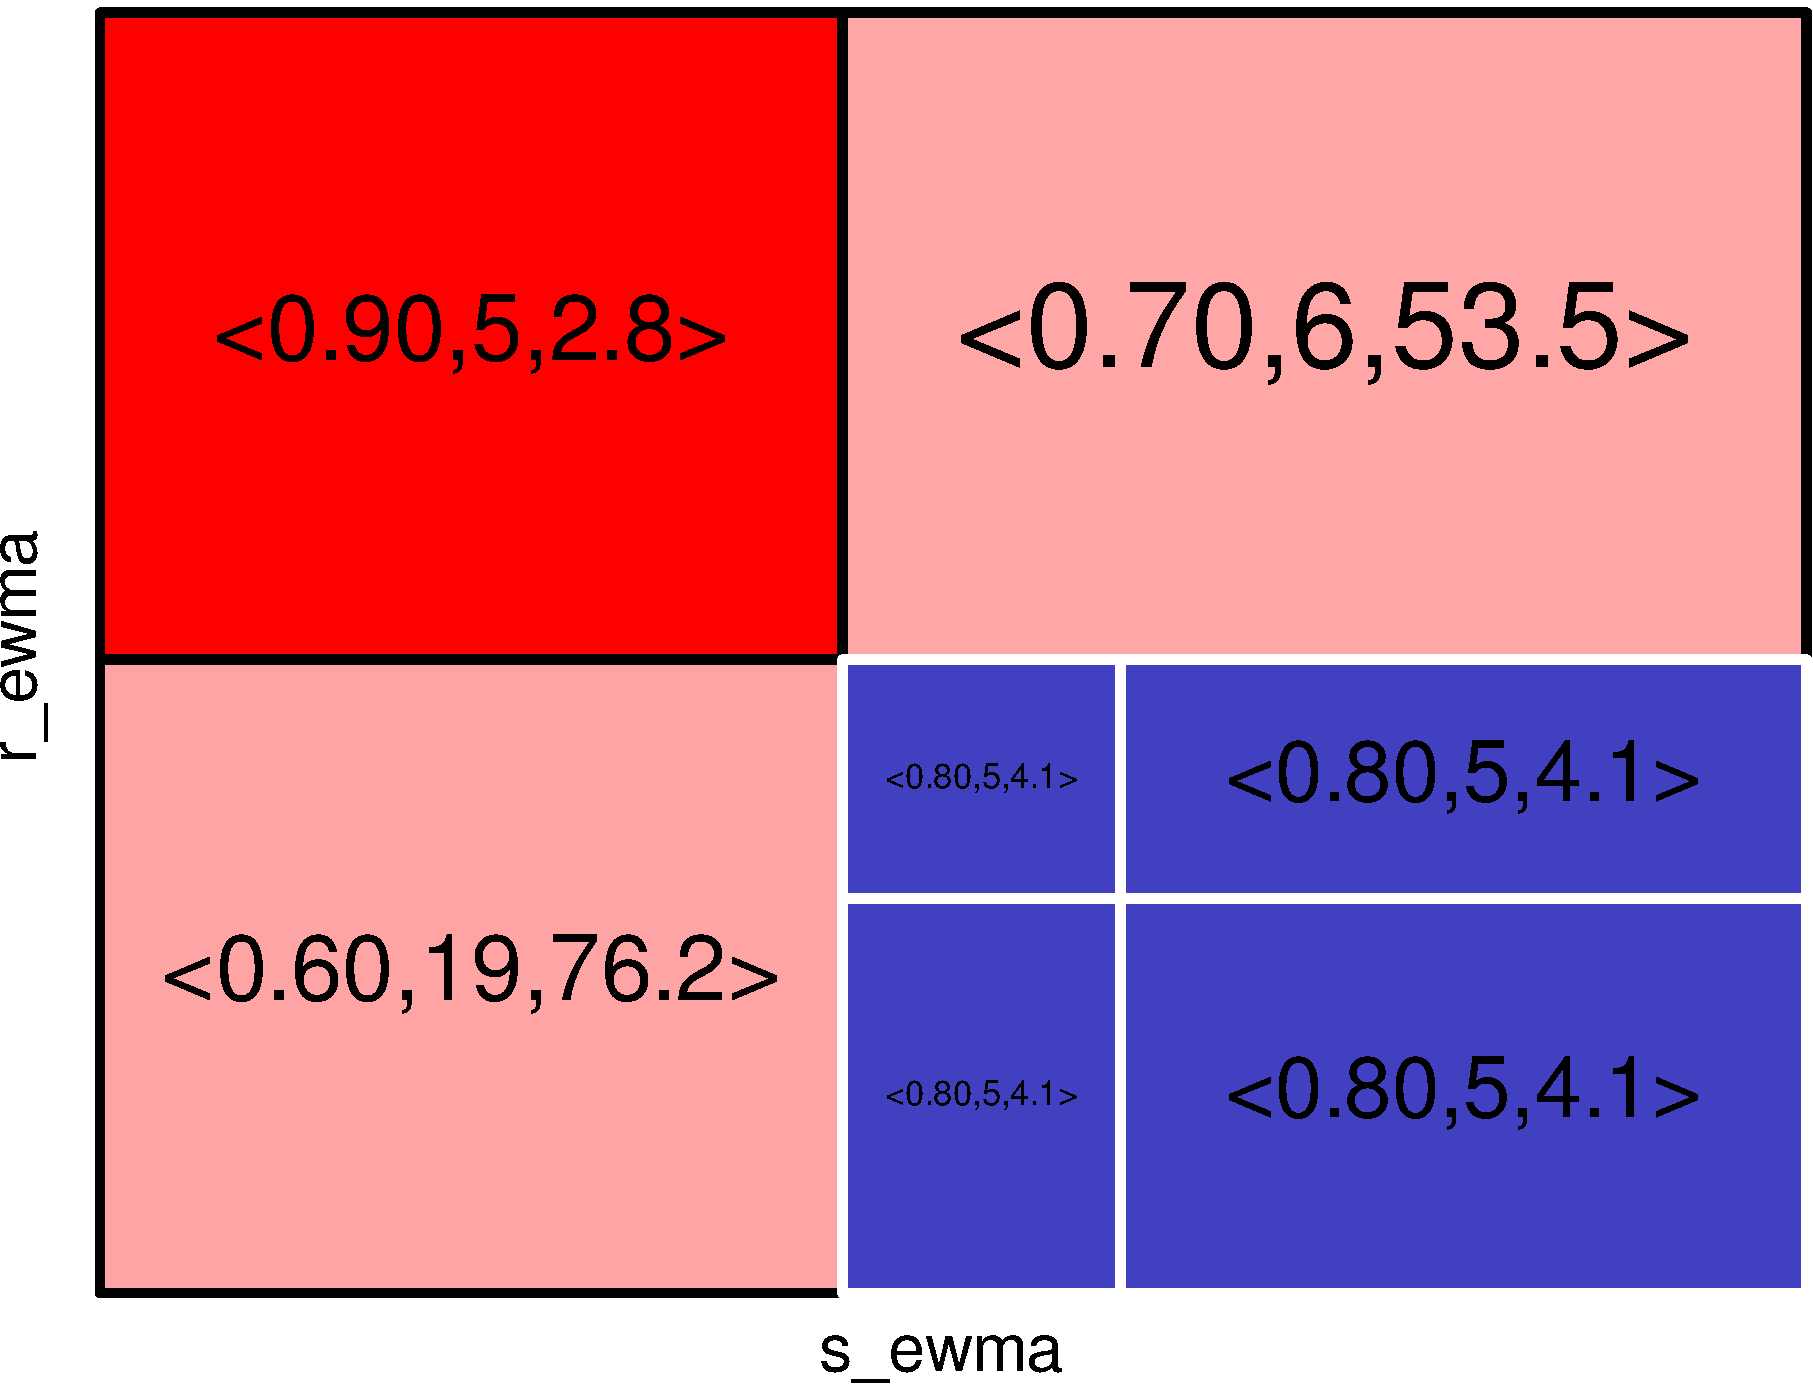
\includegraphics[width=9.25 cm]{remy-graph/graph/test5.pdf}

\end{centering}
}

\only<7>{\frametitle{Optimize}
\begin{centering}
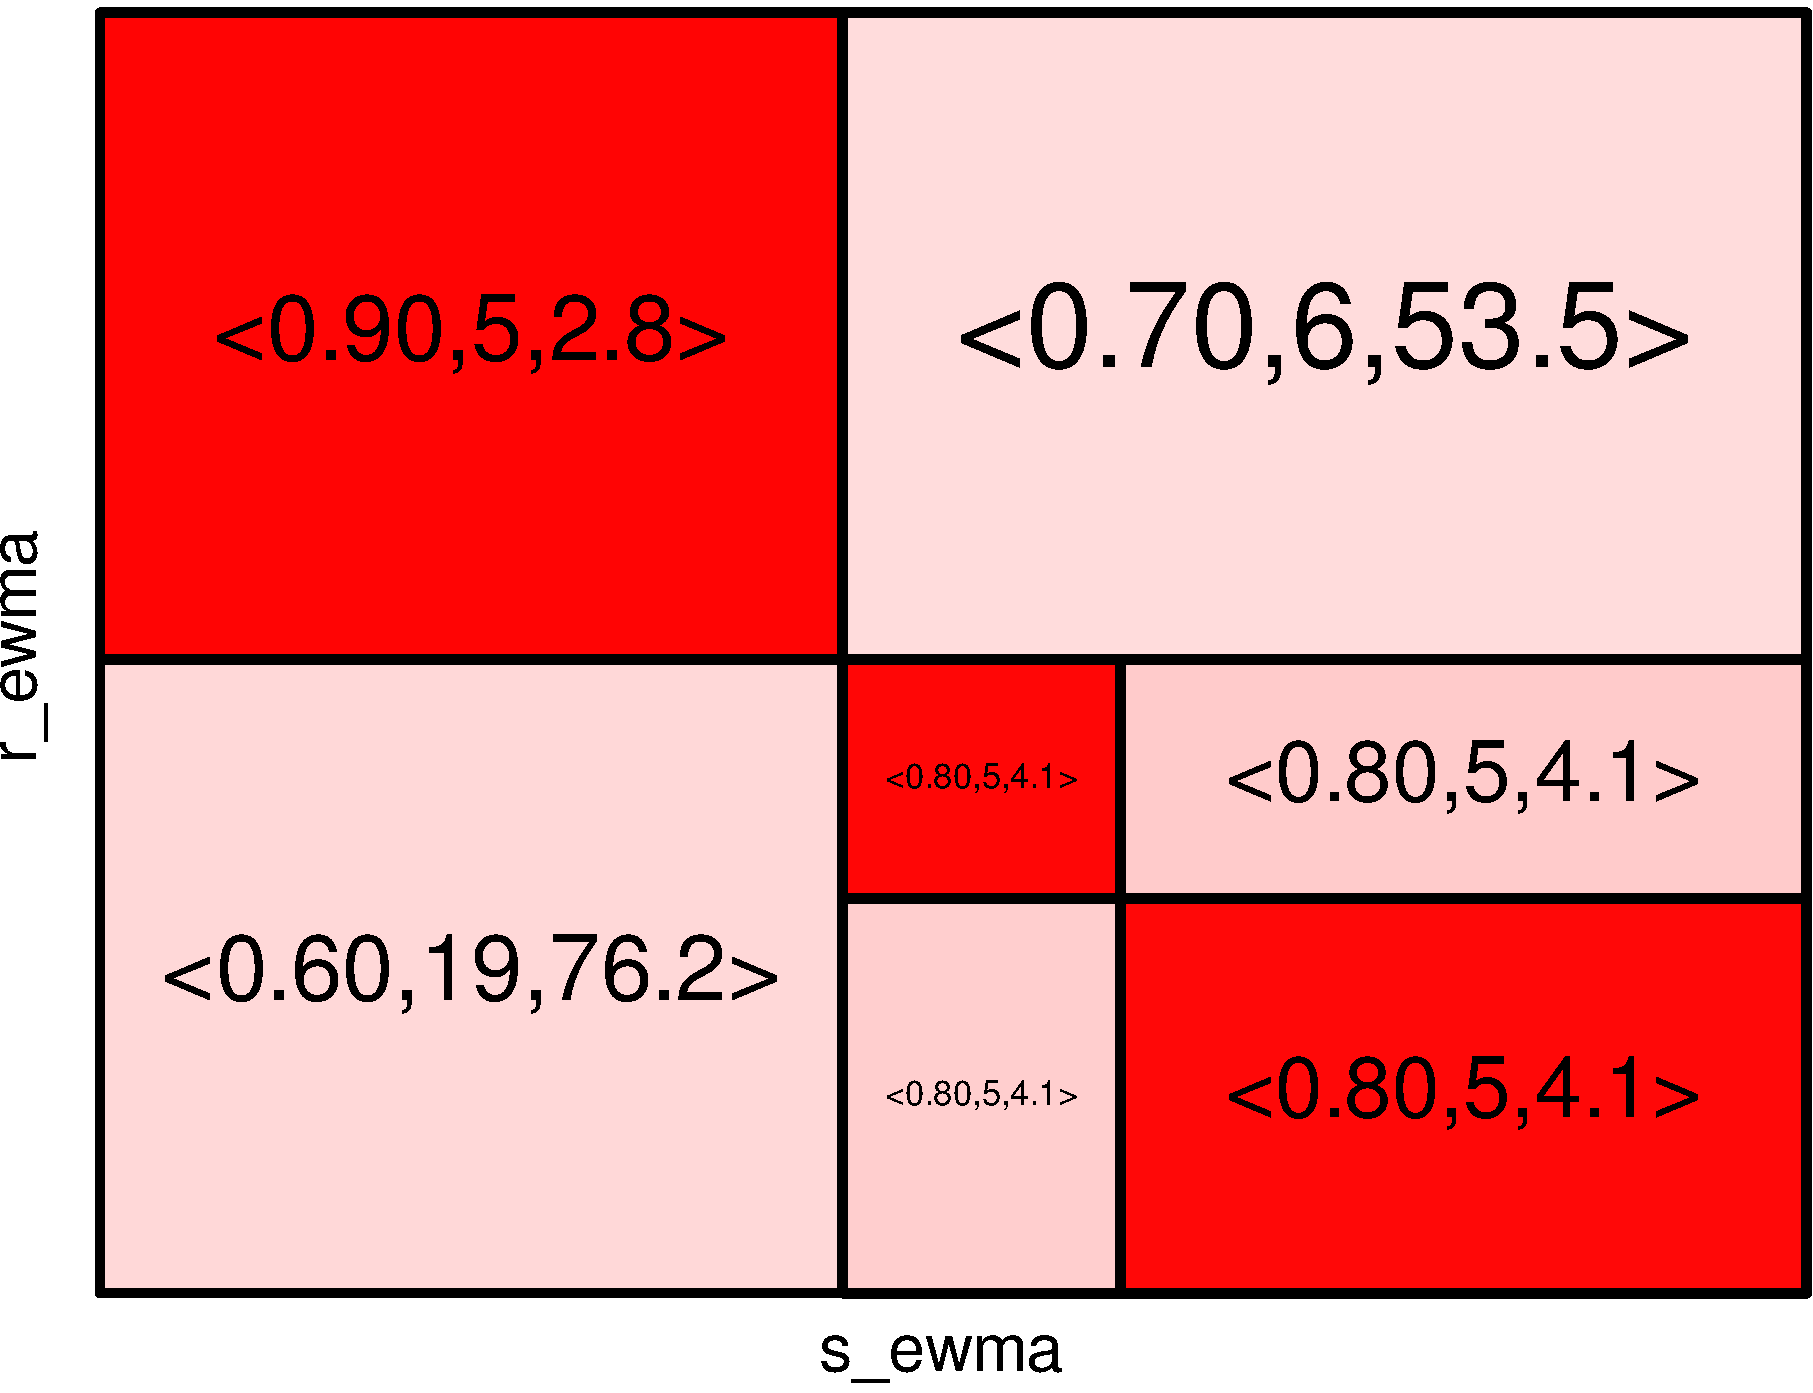
\includegraphics[width=9.25 cm]{remy-graph/graph/test6.pdf}

\end{centering}
}
\only<8>{\frametitle{Split}\begin{centering}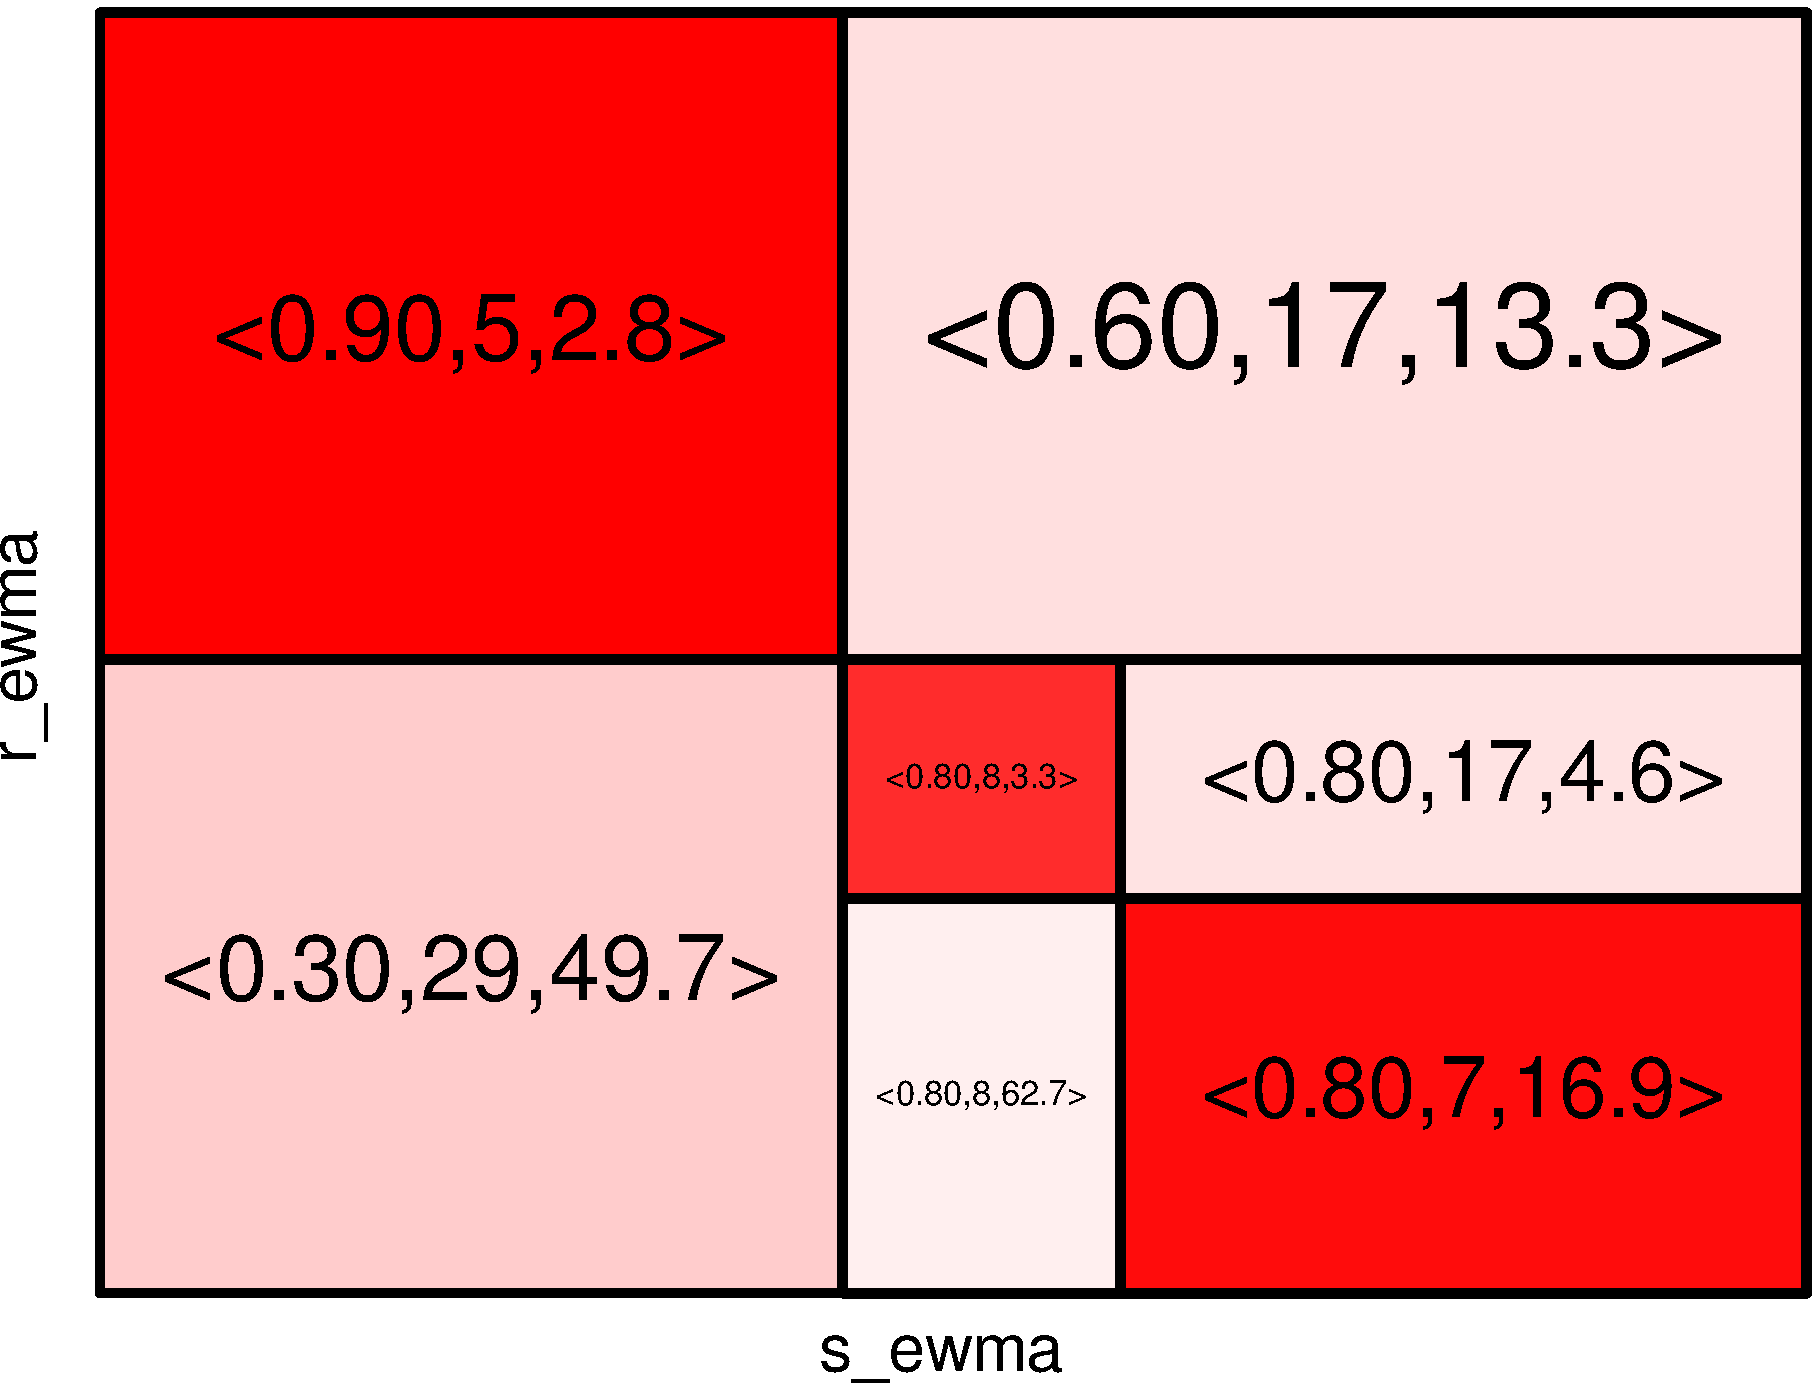
\includegraphics[width=9.25 cm]{remy-graph/graph/test7.pdf}

\end{centering}}

\only<9>{\frametitle{Simulate}\begin{centering}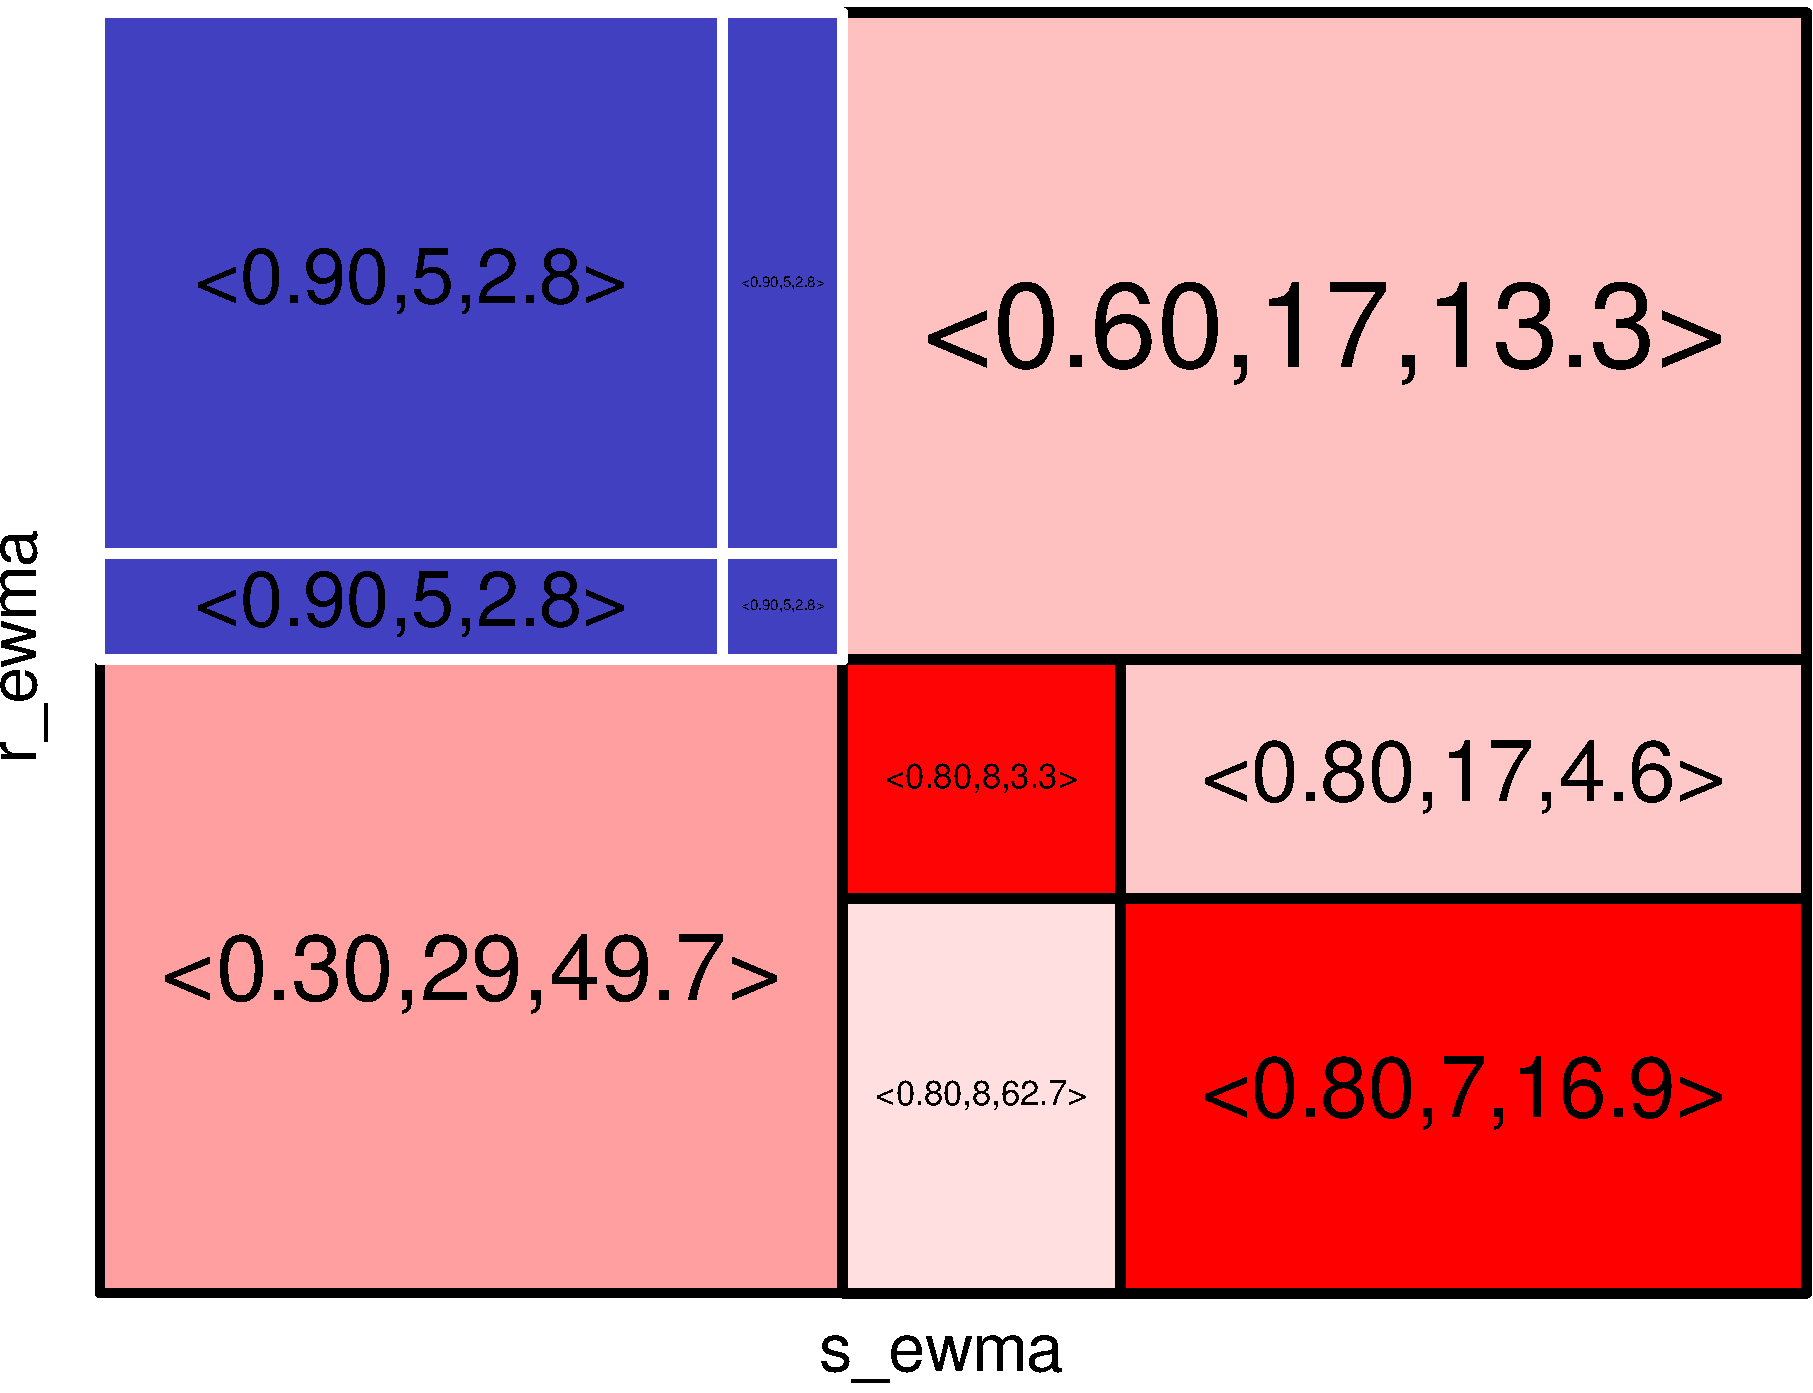
\includegraphics[width=9.25 cm]{remy-graph/graph/test8.pdf}

\end{centering}}

\end{frame}
